\chapter{One Dimensional Stochastic Case}\label{chap:oned-stochastic}

Here we return to the one dimensional version of this equation, but this time
we introduce some form of uncertainty in the coefficients of the equation:

\begin{equation}\label{eq:oned-stochastic}
  \begin{aligned}
      -\frac{d}{dx}\left[\kappa(x;\omega)\frac{d}{dx}u(x;\omega)\right] &= f(x)\,
                              &x \in  D = [-1,1]\, \omega \in \Omega \\
    u(x;\omega) &= 0 &x \in \partial D = \{-1,1\}\, \omega \in \Omega
  \end{aligned}
\end{equation}

where $\Omega$ is a probability space. In order to handle this case, we follow
a similar method to that we used in Chapter \ref{chap:oned-deterministic}
however with the introduction of the random parameter $\omega$ there is an
additional layer of complexity to deal with, as well as discretising the
physical domain we also need to be able to discretise the probability space
using a finite dimensional approximation.  This is where the generalised
polynomial chaos comes in.

Using the methodology outlined in \cite{general-poly-chaos} we can use various
polynomials in the \textit{Askey Scheme} to construct a finite dimensional
approximate representations of various random processes which when used in
conjunction with the Finite Element Method we can model the expected behaviour
of the solution process $u(x;\omega)$

\section{Weak Formulation}

\todo[inline]{Make exact all the functional spaces etc.}

As with the deterministic cases, we first need to obtain the weak formulation
of the problem, where we multiply through by $w \in W$ and integrate over the
domain.

\begin{equation}
    -\int_{\Omega}\int_{-1}^1\left(\frac{d}{dx}\left[\kappa(x;\omega)\frac{d}{dx}u(x;\omega)\right]
    w(x;\omega)\right)\, dx\, d\Omega = \int_{\Omega}\int_{-1}^1 f(x)w(x;\omega)\, dx\, d\Omega
\end{equation}

Proceeding with integration by parts

\begin{equation}
    -\int_{\Omega}\left(
      \underbrace{\left[\kappa(x;\omega)\frac{d}{dx}u(x;\omega)
                        w(x;\omega)\right]_{-1}^1}_{= 0}
       -\int_{-1}^1\kappa(x;\omega)\frac{d}{dx}u(x;\omega)\frac{d}{dx}w(x;\omega)\, dx
    \right)\, d\Omega = \int_{\Omega}\int_{-1}^1 f(x)w(x;\omega)\, dx\, d\Omega
\end{equation}

where the underbraced term is zero as the elements of $W$ are zero at the
endpoints of the domain. Hence the weak form of this equation is given by:

\begin{equation}\label{eq:wk-one-d-stochastic}
    \int_{\Omega}\int_{-1}^1\kappa(x;\omega)
           \frac{d}{dx}u(x;\omega)\frac{d}{dx}w(x;\omega)\, dx\, d\Omega =
           \int_{\Omega}\int_{-1}^1 f(x)w(x;\omega)\, dx\, d\Omega
\end{equation}

where finding a solution in this sense would be to find a $u \in V$ such that
the above is satisfied $\forall w \in W$

\section{Discrete Formulation}

Constructing a finite dimensional approximation to
\myref{eq:wk-one-d-stochastic} requires us to discretise both physical and
probability spaces. For the physical space we can proceed in a similar fashion
to Chapter \ref{chap:oned-deterministic} taking into account that the domain
now extends to include the interval $[-1, 0]$

Given a parameter $N \in \mathbb{N}$ we place $N+1$ equally spaced nodes
$x_i, i \in \{0,\ldots,N\}$ in the interval $[-1,1]$ such that $x_0= -1$,
$x_N = 1$. This subdivides the interval into $N$ subintervals
$I_i = [x_i, x_{i+1}]$, for each $i \in \{0,\ldots,N-1\}$. These subintervals
will have length $h = 1/N$ and we can define our discretisation as follows:

\[
    D^h = \bigcup_{i=0}^{N - 1}I_i
\]

Upon which we can define finite dimensional subspaces of $V$ and $W$:

\begin{align*}
    V^h &= \{v \in V : v \text{ is linear on } I_i,\ i \in \{0,\ldots,N-1\},
                    \  v \text{ is continuous on } [-1,1]\} \\
    W^h &= \{w \in W : w \text{ is linear on } I_i,\ i \in \{0,\ldots,N-1\},
                    \  w \text{ is continuous on } [-1,1]\}
\end{align*}

Then we can choose the `hat functions' as our basis again which are defined
just as they were in \myref{eq:one-d-hat-basis} hence we can approximate $f(x)$
as follows:

\begin{equation}\label{eq:oned-stochastic-f-approx}
    f(x) \approx \sum_{j=0}^Nf_j\phi_i(x)
\end{equation}

where $f_j = f(x_j)$. This also allows us to write our approximate solution
process $u^h$ as follows:

\begin{equation}\label{eq:oned-stochastic-uh}
    u^h(x;\omega) = \sum_{j=0}^Nu_j(\omega)\phi_j(x)
\end{equation}

We now have a discrete representation for $u^h$ in the physical space but now
we need to turn our attention to approximating the diffusion coefficient
$\kappa(x;\omega)$ and the stochastic parts of the solution process
$u_j(\omega)$

\subsection{Polynomial Chaos}

Much like the physical case, constructing a finite dimensional approximation to
a probability space requires choosing a set of orthogonal functions to form a
basis which spans the space. As shown in \cite{gpc} members from the
\textit{Askey Scheme} of orthogonal polynomials can be used to construct finite
dimensional approximations to second order random processes.

By introducing the following notation for the expected value of a quantity:

\begin{equation}\label{eq:oned-stochastic-expect-notation}
    \langle\cdot\rangle = \int_{\Omega}(\cdot) \,d\omega
\end{equation}

allows us to express this orthogonality relation as follows:

\begin{equation}\label{oned-stochastic-orthog-relation}
    \langle\chi_i\chi_j\rangle = \langle\chi_i\rangle^2\delta_{ij}
\end{equation}

Depending on the probability measure of a space a different set of polynomials
are used. For example if the probability measure is for a
\textit{Gaussian process} then the \textit{Hermite polynomials} are used or in
the case of a \textit{Uniform process} the \textit{Legendre polynomials} are
used. A full table outlining the correspondence of probability measures to
polynomials can be found in \cite{general-poly-chaos}

Once the set of polynomials have been determined you can approximate a random
process as follows:

\begin{equation}
    \omega(\theta) = \sum_{s=0}^P\omega_s\chi_s(\theta)
\end{equation}

where $P = (d + p)!/d!p!$ and $d$ denotes the dimensionality of the
approximation and $p$ is the highest degree of polynomial used. For example in
the case of Legendre polynomials and $d=2$, $p=2$ that gives a total of 6
terms in the expansion. We can then define the following index scheme:

\begin{equation}
  \begin{array}{c c c }
    \alpha_1 = (0,0) & \alpha_2 = (1,0) & \alpha_3 = (0,1) \\
    \alpha_4 = (2,0) & \alpha_5 = (1,1) & \alpha_6 = (0,2)
  \end{array}
\end{equation}

Then the set of basis polynomials in this case would be given by:

\begin{equation}
  \begin{array}{l l l}
    \chi_{\alpha_1} = 1 & \chi_{\alpha_2} = \xi_1 & \chi_{\alpha_3} = \xi_2 \\
    \chi_{\alpha_4} = \frac{1}{2}(3\xi_1^2 - 1) &
    \chi_{\alpha_5} = \xi_1\xi_2 &
    \chi_{\alpha_6} = \frac{1}{2}(3\xi_2^2 - 1)
  \end{array}
\end{equation}


Therefore we may now rewrite our approximation to the solution process
\myref{eq:oned-stochastic-uh} as follows:

\begin{equation}\label{eq:oned-stochastic-uhp}
    u^{h,P}(x;\omega) = \sum_{j=0}^N\sum_{s=1}^Pu_{j,s}\chi_s(\xi)\phi_j(x)
\end{equation}

\subsection{The Karhunen-Loeve Expansion}

The Karhunen-Loeve (KL) expansion allows us to write any second order
stochastic process $X(\v{x},\omega)$ in the following way:

\begin{equation}
    X(\v{x}, \omega) = \bar{X}(\v{x})
    + \sum_{n = 0}^\infty\sqrt{\lambda_n}\beta_n(\v{x})\xi_n(\omega)
\end{equation}

where:

\begin{itemize}
    \item $\bar{X}(\v{x})$ denotes the expected value of the process
    \item $\{\xi_n(\omega)\}_{n=0}^\infty$ forms a set of uncorrelated random
          variables
    \item $\lambda_n$, $\beta_n(\v{x})$ denote the eigenvalues/eigenfunctions
          of the following eigenvalue problem:
          \[
                \int_DC(\v{x}_1, \v{x}_2)\beta(\v{x})\, d\v{x}_1
                = \lambda\beta(\v{x}_2)
          \]
          where $C(\v{x}_1,\v{x}_2)$ denotes the correlation function of the
          random process.
\end{itemize}

The derivation of this representation is discussed in \cite{stochastic-fem} as
well as a number of its properties. One such property which is useful for our
purposes is that this representation is optimal in the sense that when we
truncate the series to a finite number of terms the mean squared error is
minimised.

Of course since this representation requires that we know the correlation
function of the random process so this will only be useful for expanding the
term $\kappa(x;\omega)$ in \myref{eq:oned-stochastic}.

For the purposes of this project we will assume that $\kappa(x;\omega)$ is
uniformly distributed between the values $a$ and $b$ with mean $\mu$,
variance $\sigma^2$ and correlation function given by:

\begin{equation}
    C(x, y) = \sigma^2\exp\left(-\frac{|x - y|}{k}\right)
\end{equation}

where $k$ is the correlation length that for simplicity we set to $1$.
Therefore to determine $\beta_n, \lambda_n$ we have to solve the following
integral equation:

\begin{equation}\label{eq:oned-stochastic-kle-eigenvalue-problem}
    \sigma^2\int_{-1}^1\exp(-|x - y|)\beta_n(y) dy = \lambda_n\beta_n(x)
\end{equation}

A detailed discussion on finding the eigenvalues/eigenfunctions above can be
found in \cite{stochastic-fem} but solving this numerically will be sufficient
for our purposes. Therefore we will be able to approximate $\kappa(x;\omega)$
as follows:

\begin{equation}\label{eq:oned-stochastic-kl-kappa}
    \kappa(x;\omega) \approx
        \mu + \sigma^2\sum_{l=1}^d\sqrt{\lambda_l}\beta_l(x)\xi_l(\omega)
\end{equation}

\subsubsection{Obtaining a Numeric Representation of the KL Expansion}

Unfortunately I was unable to find an existing method to numerically solve
\myref{eq:oned-stochastic-kle-eigenvalue-problem} using Python however this is
a relatively easy problem to solve in Matlab once you make use of the
\textit{Chebfun} numerical computation library \cite{chebfun}. The Matlab code
which solves this problem can be found in Listing \ref{code:matlab-eigen}.

\begin{lstlisting}[caption={Matlab code which finds the first 5 eigenvalues and
                            associated eigenfunctions},
                   label={code:matlab-eigen},
                   language=Matlab]
function KLEigs(k)
    K = @(x, y) exp(-abs(x-y));
    L = chebop(@(u) fred(K,u));
    [V,D] = eigs(L, k, 'lm');

    values = diag(D);
    dlmwrite('expansion-data.csv', transpose(values), ',');

    for i = 1:len(values)
        dlmwrite('expansion-data.csv', transpose(V{1,i}.points), '-append', 'delimiter', ',');
        dlmwrite('expansion-data.csv', transpose(V{1,i}.values), '-append', 'delimiter', ',');
    end
end
\end{lstlisting}

In order to be able to use the results from Matlab in the remaining Python
code, we require a brief discussion of how the \textit{Chebfun} library
represents mathematical functions. As stated in \cite{chebfun-data}, the
fundamental data structure \incode{chebfun} is a numerical representation of a
function $f$ using a set of numbers $\{f_0, \ldots, f_N\}$ where $f_j = f(x_j)$
, $j \in \{0, \ldots, N\}$ where the $x_j$ are particular points in the domain
called Chebyshev points. When the $f_j$ are used in conjunction with
\textit{baycentric interpolation} one can achieve a good, fast and stable
approximation to $f$.

Therefore in order to use the Matlab results in our Python we simply need to
export the $f_j$, $x_j$ of each of the eigenfunctions we find. Then by using
the \incode{BarycentricInterpolator} that is part of the \textit{scipy} library
\cite{scipy} we can reconstruct the functions in our Python code. The code
which performs this reconstruction can be found in Listing
\ref{code:python-reconstruct-eigen}.

\begin{lstlisting}[caption={Python code which reconstructs the eigenfunctions
                            we found using Matlab},
                   label={code:python-reconstruct-eigen},
                   language=Python]
import csv
import scipy.interpolate import BarycentricInterpolator


def reconstruct_eigenfunctions(filename):
    """
    Given a filename, read the CSV data and reconstruct the eigenfunctions
    as they are represented by the Matlab code
    """

    # Read and parse the CSV data
    with open(filename) as f:
        reader = csv.reader(f)
        rows = [row for row in reader]

    # Eigenvalues are given by the first row of data
    eigenvalues = [float(l) for l in rows[0]]

    data = list()

    for i in range(len(eigenvalues)):

        # The remaining rows alternate between the x_j and f(x_j)
        # representing the i-th eigenfunction associated with the i-th eigenvalue
        p = BarycentricInterpolator([float(x) for x in rows[2*i + 1]],
                                    [float(y) for y in rows[2*i + 2]])

        data.append({'lambda': eigenvalues[i],
                     'beta': p})

    # Reverse the list so the eigenvalues are sorted from largest - smallest
    data.reverse()

    return data
\end{lstlisting}

Finally it is worth considering if this process does indeed give the right
result, thankfully as this particular correlation function
\myref{eq:oned-stochastic-kle-eigenvalue-problem} is discussed in
\cite{stochastic-fem} we can compare results. Hence as Figure
\ref{fig:kle-eigenfunctions} matches what we see in Figure $2.1$ in
\textit{Ghanem \& Spanos}, we can be confident that indeed we have obtained the
correct results.

\begin{figure}
    \centering
    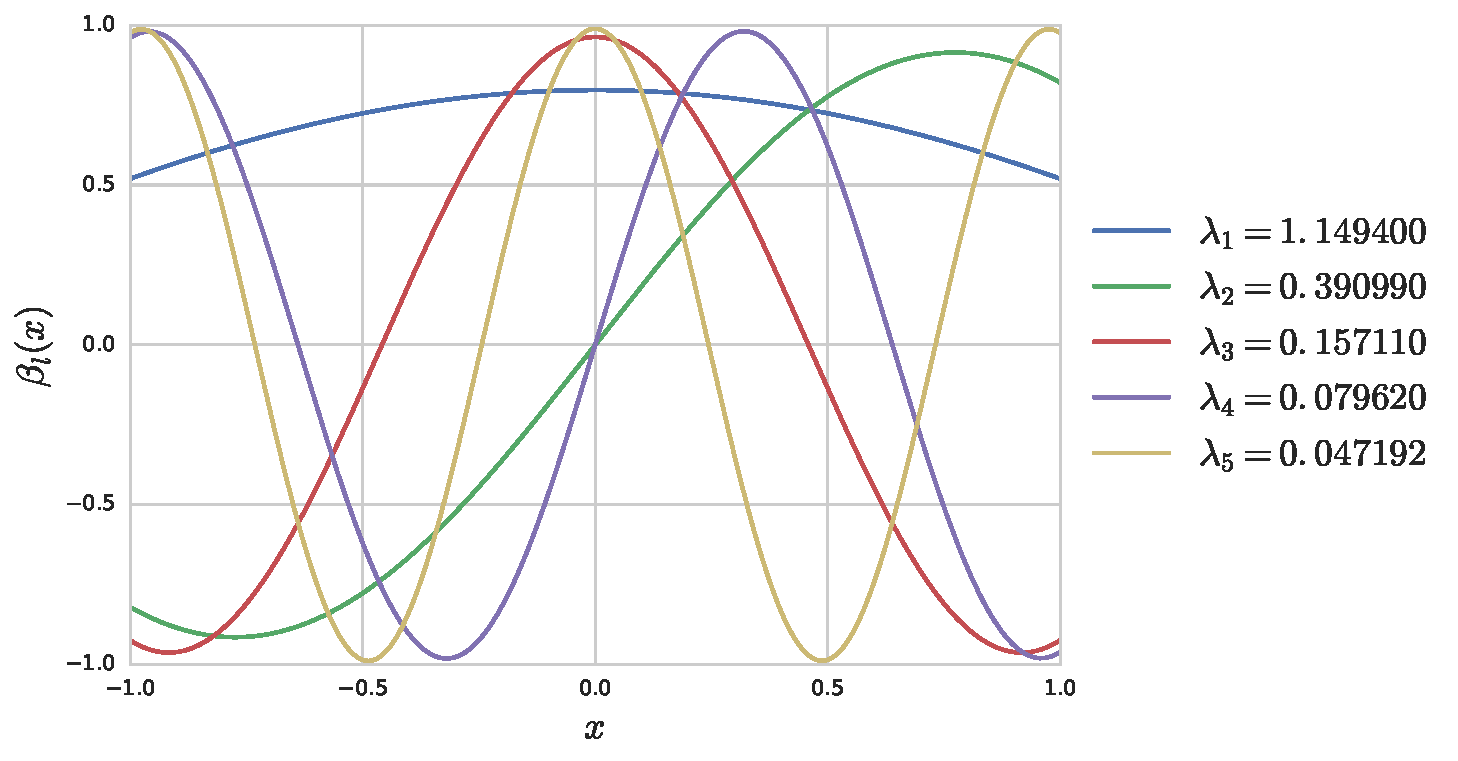
\includegraphics[width=0.7\textwidth]{img/kle-eigenfunctions.pdf}
    \caption{The first 5 eigenfunctions and associated eigenvalues of
             \myref{eq:oned-stochastic-kle-eigenvalue-problem}}
    \label{fig:kle-eigenfunctions}
\end{figure}

\subsection{Derivation of Global System of Equations}

Since the weak formulation \myref{eq:wk-one-d-stochastic} has to be satisifed
$\forall w \in W$ it must in particular hold for the basis functions. So by
using the expansions \myref{eq:oned-stochastic-uhp},
\myref{eq:oned-stochastic-f-approx} and \myref{eq:oned-stochastic-kl-kappa} and
choosing $w = \phi_i(x)\chi_t(x)$ for each $i = \{0,\ldots,N\}$ and each $t =
\{0,\ldots,P\}$ and substituting into \myref{eq:wk-one-d-stochastic} we
obtain:

\begin{align*}
    \int_{\Omega}\int_{-1}^1
      \left(\mu + \sum_{l=1}^d\sqrt{\lambda_l}\beta_l(x)\xi_l(\omega)\right)
      \frac{d}{dx}\left(\sum_{j=0}^N\sum_{s=1}^Pu_{s,j}\phi_j(x)\chi(\omega)\right)
      \phi_i'(x)\chi_t(\omega)\, dx\, d\Omega \\ =
    \int_{\Omega}\int_{-1}^1
      \left(\sum_{j=0}^Nf_j\phi_j(x)\right)
      \phi_i(x)\chi_t(\omega)\, dx\, d\Omega
\end{align*}

Then by the linearity of the integral and differential operator and taking
advantage of our notation for the expectation
\myref{eq:oned-stochastic-expect-notation} we may write this as:

\begin{align}\label{eq:oned-stochastic-discrete}
  \begin{split}
      \sum_{j=0}^N\sum_{s=0}^Pu_{s,j}\left[
          \mu\expect{\chi_s\chi_t}
          \int_{-1}^1\phi_j'(x)\phi_i'(x)\, dx +
          \sum_{l=1}^d\sqrt{\lambda_l}\expect{\xi_l\chi_s\chi_t}
          \left(\int_{-1}^1 \beta_l(x)\phi_j'(x)\phi_i(x)\, dx\right)
      \right]\\ =
      \sum_{j=0}^N\sum_{s=0}^Pf_j\expect{\chi_s\chi_t}
          \left(\int_{-1}^1\phi_j(x)\phi_i(x)\, dx\right)
  \end{split}
\end{align}

for each $j \in \{0,\ldots,N\}$ and each $t \in \{0,\ldots,P\}$. Just as in
the deterministic case, we know the solution at the endpoints due to the
boundary conditions on the problem \myref{eq:oned-stochastic} hence we can
remove the terms associated with $j = 0$ and $j = N$ from the system of
equations. Then by defining the $i$-th, $j$-th component of the matrix
$A_{s,t}$ to be the terms in the square brackets of
\myref{eq:oned-stochastic-discrete} and the $i$-th, $j$-th component of the
matrix $M_{s,t}$ we obtain the following:

\begin{equation}
    \sum_{j=1}^{N - 1}\sum_{s=0}^P(A_{s,t})_{i,j}u_{s,j} =
    \sum_{j=0}^N\sum_{s=0}^P(M_{s,t})_{i,j}f_j
\end{equation}

for $i \in \{1,\ldots,N - 1\}$ and $t \in \{0,\ldots,P\}$. Which defines a
$(N - 1)P \times (N - 1)P$ system of linear equations $A\v{u} = M\v{f}$ in
which the global stiffness matrix $A$ takes the following form:

\begin{equation}
    A = \left[\begin{array}{c c c}
            A_{1,1} & \cdots & A_{1,P} \\
            \vdots & & \vdots \\
            A_{P,1} & \cdots & A_{P,P}
        \end{array}\right]
\end{equation}

where each $A_{s,t}$ are $(N - 1) \times (N - 1)$ matrices. Similarly the
global mass matrix $M$ takes the form:

\begin{equation}
    M = \left[\begin{array}{c c c}
            M_{1,1} & \cdots & M_{1,P} \\
            \vdots & & \vdots \\
            M_{P,1} & \cdots & M_{P,P}
        \end{array}\right]
\end{equation}

where each $M_{s,t}$ are $(N - 1) \times (N + 1) $ matrices.

\section{Constructing the Global System}

In order to construct the global system of equations we need to determine the
form of each of the smaller matrices $A_{s,t}$ and $M_{s,t}$

\subsection{The Global Stiffness Matrix}

\subsubsection{Matrices on the Diagonal}

By setting $s=t$ in \myref{eq:oned-stochastic-discrete} we obtain the following
expression for the entries of the matrices sitting on the diagonal of the
global stiffness matrix:

\begin{equation}
    A_{s,s} = \sum_{j=1}^{N-1}\left(\mu\expect{\chi_s^2}
        \int_{-1}^1 \phi_j'(x)\phi_i'(x)\, dx
       + \sum_{l=1}^d\sqrt{\lambda_n}\expect{\xi_l\chi_s^2}
       \int_{-1}^1 \beta_l(x)\phi_j'(x)\phi_i'(x) \, dx\right)
\end{equation}

for each $i \in \{1,\ldots,N-1\}$. Now if we consider the quantity
$\expect{\xi_l\chi_s^2}$ for a moment as the function $\chi_s^2$ is even and
$\xi_l$ is an odd function their product is odd therefore, as we are integrating
over a symmetric domain, this quantity vanishes. Hence the above reduces to:

\begin{equation}
    A_{s,s} = \mu\expect{\chi_s^2}\sum_{j=1}^{N - 1}\left(\int_{-1}^1
                \phi_j'(x)\phi_i'(x)\, dx\right)
\end{equation}

for each $i \in \{1,\ldots,N-1\}$. As the quantity $\mu\expect{\chi_s^2}$ is
fully deterministic and scalar if we compare this with Chapter
\ref{chap:oned-deterministic} we can treat this similarly. So by setting $a =
\mu\expect{\chi_s^2}, b = 0, c = 0$ in \myref{eq:oned-deterministic-discrete}
and following a similar argument as outlined in Section
\ref{sec:oned-deterministic-local-stiffness} we obtain the following form of
the local stiffness matrix $A_{s,s}^{(k)}$:

\begin{align}\label{eq:oned-stochasic-local-stifness-diag}
  \begin{split}
    A_{s,s}^{(k)} &= \frac{\mu\expect{\chi_s^2}}{h_k}\left[\begin{array}{c c}
                1 & -1 \\ -1 & 1
              \end{array}\right] \\
    &= \frac{2\mu}{h_k(2s + 1)}\left[\begin{array}{c c}
              1 & -1 \\ -1 & 1
      \end{array}\right]
  \end{split}
\end{align}

where $\expect{\chi_s^2} = \frac{2}{2s + 1}$ is the orthogonality relation for
the \textit{Legendre Polynomials} \cite{poly-bible}. Continuing with the same
argument as in Section \ref{sec:oned-deterministic-global-stiffness-assembly}
we find that the matrix $A_{s,s}$ will have the form as shown in
\myref{eq:oned-deterministic-global-stiffness}.

\subsubsection{The Off-Diagonal Matrices}

Now if we consider the case where $s \neq t$ in
\myref{eq:oned-stochastic-discrete} we obtain:

\begin{equation}\label{eq:oned-stochastic-off-diagonal-stiffness}
    A_{s,t} = \sum_{j=1}^{N - 1}\left(\mu\expect{\chi_s\chi_t}
        \int_{-1}^1 \phi_j'(x)\phi_i'(x)\, dx
       + \sum_{l=1}^d\sqrt{\lambda_n}\expect{\xi_l\chi_s\chi_t}
       \int_{-1}^1 \beta_l(x)\phi_j'(x)\phi_i'(x)\, dx\right)
\end{equation}

for each $i \in \{1,\ldots,N-1\}$. By the orthogonality relation
$\expect{\chi_s\chi_t} = \expect{\chi_s^2}\delta_{st}$, the first term vanishes
and we are left with:

\begin{equation}
    A_{s,t} = \sum_{j=1}^{N - 1}\left(
        \sum_{l=1}^d\sqrt{\lambda_n}\expect{\xi_l\chi_s\chi_t}
            \int_{-1}^1\beta_l(x)\phi_j'(x)\phi_i'(x)\, dx\right)
\end{equation}

\subsection{The Global Mass Matrix}

\subsubsection{Matrices on the Diagonal}

As with the global stiffness matrix we will first consider the matrices sat on
the main diagonal. By setting $s = t$ in \myref{eq:oned-stochastic-discrete} we
obtain the following expression:

\begin{equation}
    M_{s,s} = \sum_{j=0}^Nf_j\expect{\chi_s^2}\left(
        \int_{-1}^1\phi_j(x)\phi_i(x)\, dx\right)
\end{equation}

for each $i \in \{1,\ldots,N-1\}$. The quantity $f_j\expect{\chi_s^2}$ is now
fully deterministic and scalar so proceeding with a similar argument as in
Section \ref{sec:oned-deterministic-local-mass} we find that the local mass
matrix for the matrix $M_{s,s}$ is given by:

\begin{align}
  \begin{split}
    M_{s,s}^{(k)} &= \frac{\expect{\chi_s^2}h_k}{6}\left[\begin{array}{c c}
                        2 & 1 \\ 1 & 2
                    \end{array}\right]\\
                  &= \frac{h_k}{3(2s + 1)}\left[\begin{array}{c c}
                        2 & 1 \\ 1 & 2
                    \end{array}\right]
  \end{split}
\end{align}

where we again use the orthogonality relation of the \textit{Lengendre
Polynomials}. Continuing with a similar argument to Section
\ref{sec:oned-deterministic-global-mass-assembly} we find that the matrix
$M_{s,s}$ will have the form found in \myref{eq:oned-deterministic-global-mass}

\subsubsection{The Off-Diagonal Matrices}

Now when we consider the case where $s \neq t$,
\myref{eq:oned-stochastic-discrete} redcues to:

\begin{equation}
    M_{s,t} = \sum_{j=0}^Nf_j\expect{\chi_s\chi_t}\left(
        \int_{-1}^1\phi_j(x)\phi_i(x)\, dx
    \right)
\end{equation}

for each $i \in \{1,\ldots,N - 1\}$By the orthogonality relation
$\expect{\chi_s\chi_t} = \expect{\chi_s^2}\delta_{st}$ all terms in the off
diagonal matrices vanish.

Therefore the global mass matrix is of the form:

\begin{equation}
    M = \left[\begin{array}{c c c c}
            M_{1,1} & 0 & \cdots & 0 \\
            0 & M_{2,2} & \cdots & 0 \\
            \vdots & & & \vdots \\
            0 & \cdots & 0 & M_{P,P}
    \end{array}\right]
\end{equation}
